\section{Findings} % (fold)
\label{sec:findings}
With each approach we generate topics for the \crowdre{} dataset. In accordance with the predefined application domain labels, we expect to find four different topics: \textit{Energy, Entertainment, Health} and \textit{Safety}. Sentences labeled as \textit{Other} are assumed to be visible as noise in the result.
In our plots, we always plot the different requirement sentences. We use t-SNE to transform the embeddings into 2-dimensional space for our plots\,\cite{maaten_visualizing_2008}. The coloring is based on the application domain the requirements are associated with and is as follows: \textcolor{clr_energy}{\emph{Energy}}, \textcolor{clr_entertainment}{\emph{Entertainment}}, \textcolor{clr_health}{\emph{Health}}, \textcolor{clr_safety}{\emph{Safety}} and \textcolor{clr_other}{\emph{Other}}.

\subsection{LDA} % (fold)
\label{sub:findings_lda}

Unfortunately, the result of the LDA doesn't match the expected topics. The approach itself creates some separable clusters, they can not be mapped to the expected ones considering the soft labeled domains. Still, some similarity between the requirements that are plotted next to each other can be found.

The processing time of the LDA approach is very fast which means the performance of is very good compared to approaches with high computational effort. The overall result for the LDA approach is that we couldn't gather the expected topics from the given dataset. 

\subsection{word2vec \& PCA} % (fold)
\label{sub:findings_w2v}
As shown in \autoref{fig:w2v-pretrained-4}, we can identify two clusters in the plot that results from combining word2vec and dimensionality reduction (PCA). As with most machine learning techniques, it is difficult to say though, why our approach resulted in these two clusters exactly\,\cite{ribeiro_why_2016}. To better understand our results, we perform a shallow analysis of the plotted sentences nonetheless and find the following:
\begin{enumerate}
  \item Sentences with multiple words in common are plotted in close proximity to each other\footnote{E.g. \textit{``As a home owner I want Room thermostat sensor so that The room is optimal temperature for an occupant''} at (28.492, -28.309) and \textit{``As a home occupant I want Room thermostats so that Protect the room temperature''} at (28.607, -28.423)}.
  \item Sentences with fewer words in common are plotted further away from each other\footnote{E.g. \textit{``As a home occupant I want music to be played when I get home so that it will help me relax''} at (29.688, 2.965) and \textit{``As a home owner I want music to play whenever I am in the kitchen so that I can be entertained while cooking or cleaning''} at (-13.520, -4.935)}.
\end{enumerate}
With (2) being a logical consequence of (1), it is important to note how (2) also applies to sentences that express related requirements in different words. This is expected to some extent, due to the shortcomings of word2vec mentioned in \autoref{sub:word_movers_distance}. Therefore, we can not model the topics as desired. Nevertheless, this approach delivers a deeper insight into the dataset already and needs relatively little computation time, as the results are available within a few minutes.

\begin{figure}[ht]
  \begin{center}
    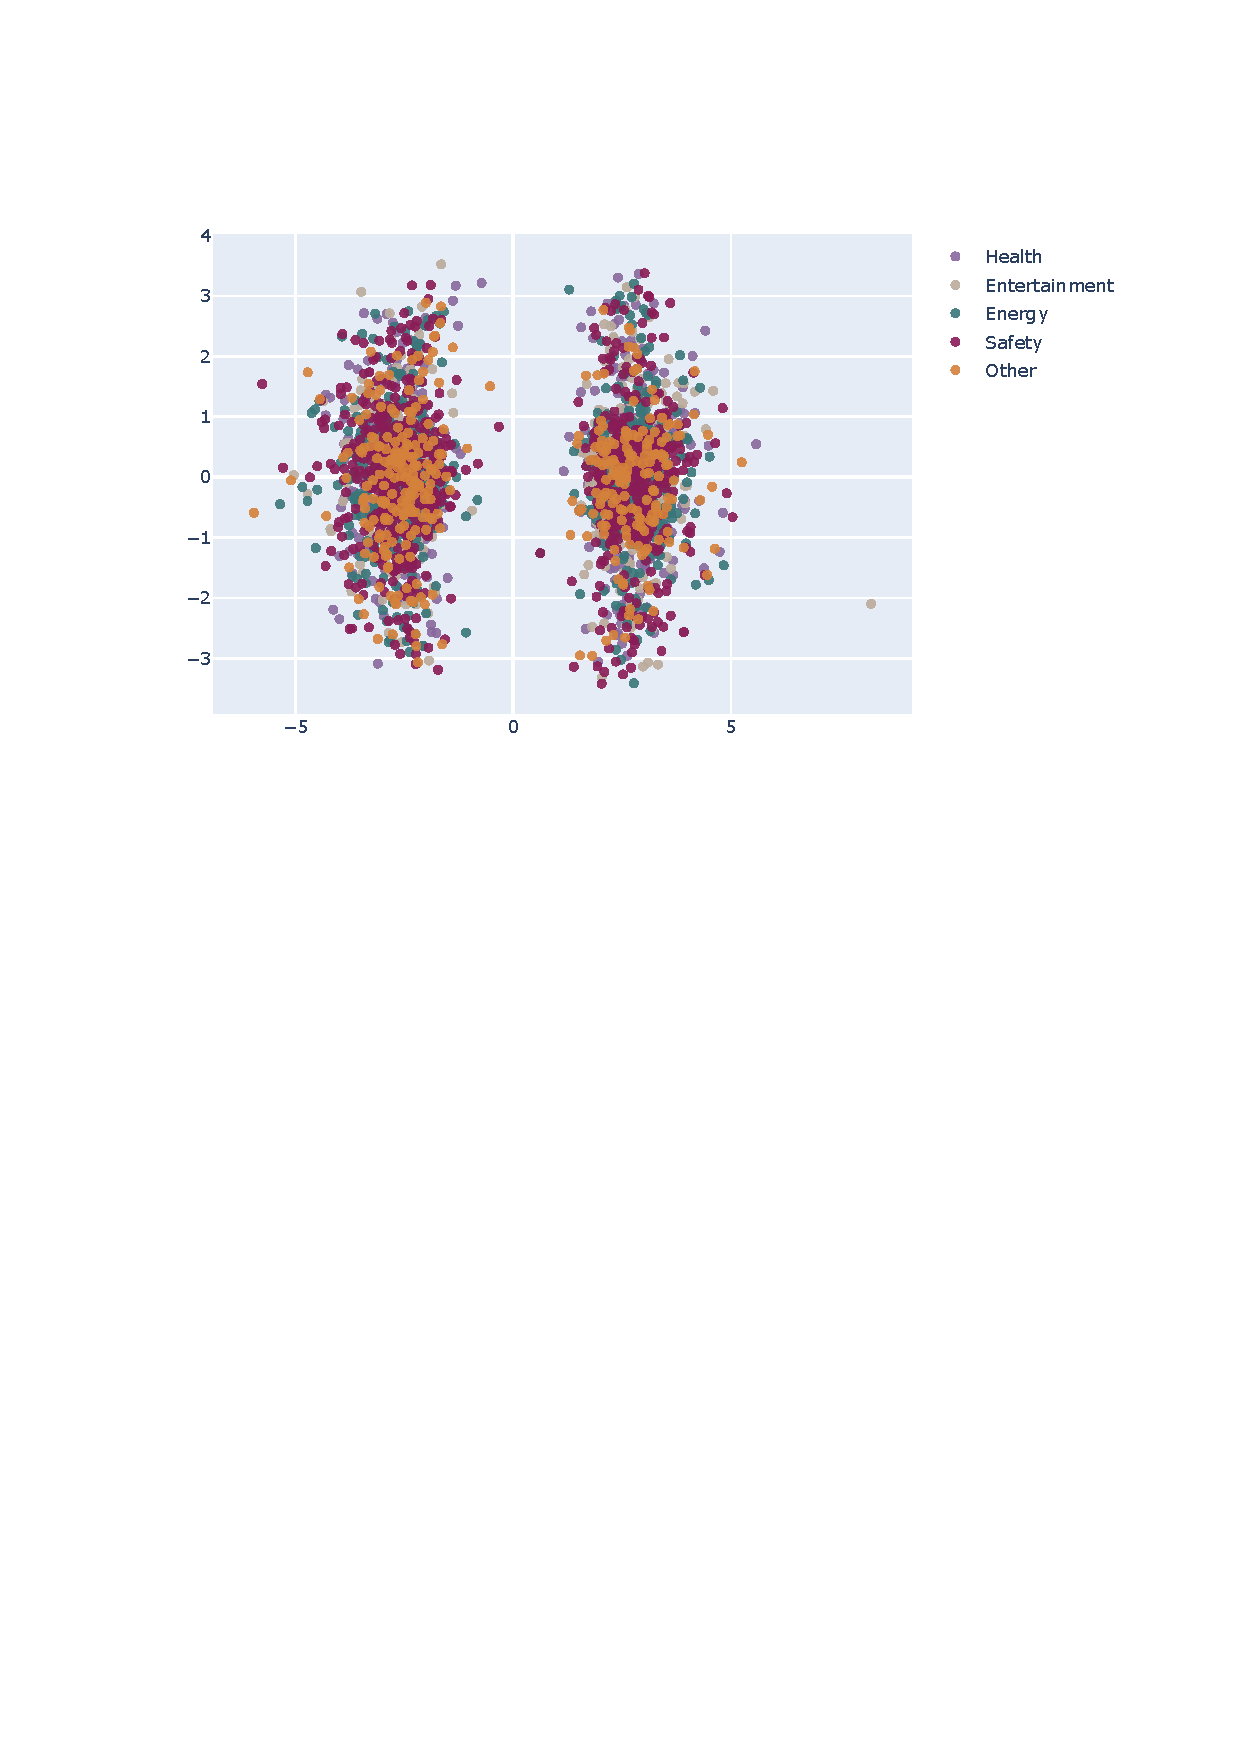
\includegraphics[width=\textwidth]{figures/word2vec_pretrained_pca-legend.pdf}
    \caption{word2vec result of the clustering using Google News word vectors}
    \label{fig:w2v-pretrained-4}
  \end{center}
\end{figure}
\FloatBarrier

\subsection{word2vec \& Word Mover's Distance} % (fold)
\label{sub:findings_wmd}
We achieve the best results using word2vec and WMD. \autoref{fig:wmd-comparison} shows plots of the distance matrices we created, as described in \autoref{sub:word_movers_distance}. With this approach we can successfully distinguish clusters both spatially and as regards content. Looking at the results in \autoref{fig:wmd-selftrained-1}, we can see that the domains \textit{Entertainment} (gray sentences around (0,0)) and \textit{Energy} (stretching from (0,-45) to (10,57)) can be well distinguished. Also, a cluster predominantly consisting of \textit{Health} sentences becomes apparent in the region from (0,20) to (70,45).\\

Judged by the pre-labeling only, it seems the clustering with our self-trained word vectors worked better. But manual inspection shows that the clustering based on the Google News vectors also brings new insights in the dataset: In \autoref{fig:wmd-pretrained-1} we can see, how the demarcation between the clusters is a lot clearer. Also, even though the sentences seem unrelated at first (told by the different label colors), the rightmost cluster\footnote{the area between (45,-15) and (75,30)} mostly contains sentences related to parenting and children. Furthermore, the topmost cluster between (20,45) and (40,65) contains requirement sentences about animals. It becomes apparent, that the dataset may be actually clustered into different clusters than the 4 domain-based clusters we initially anticipated. The higher quality of these results comes with a drawback of performance, though. On a current Intel i5-9600K 6-core processor with 3.7 GHz and 32 GB of memory attached, the calculation of the Word Mover's Distance matrix took approx. 45 minutes (even after splitting up the calculation to be done in 12 parallel threads and making use of the symmetry of the WMD).


\begin{figure}[hbt]
	\centering
	\subfigure[Self-trained word vectors\label{fig:wmd-selftrained-1}]{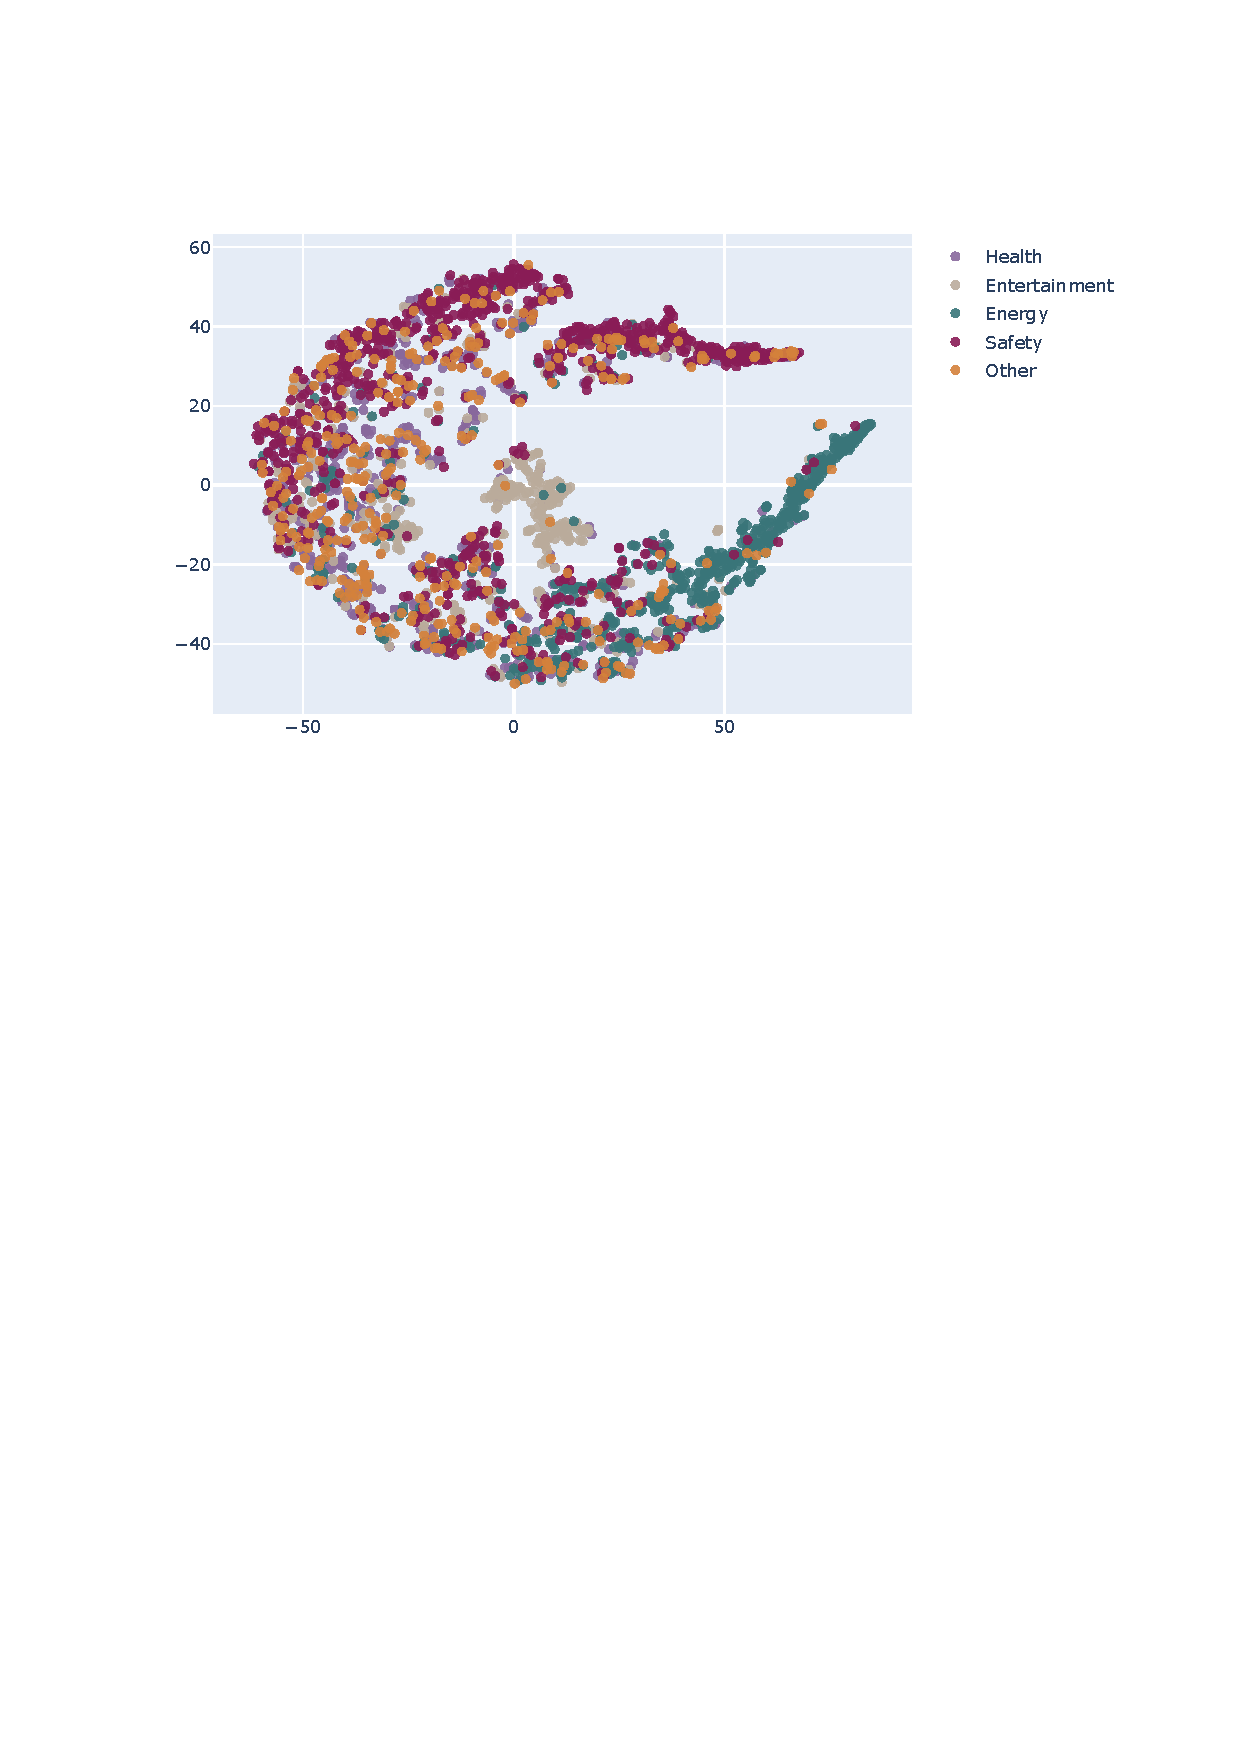
\includegraphics[width=0.49\textwidth]{figures/wmd_self_trained.pdf}}
    \subfigure[Google News word vectors\label{fig:wmd-pretrained-1}]{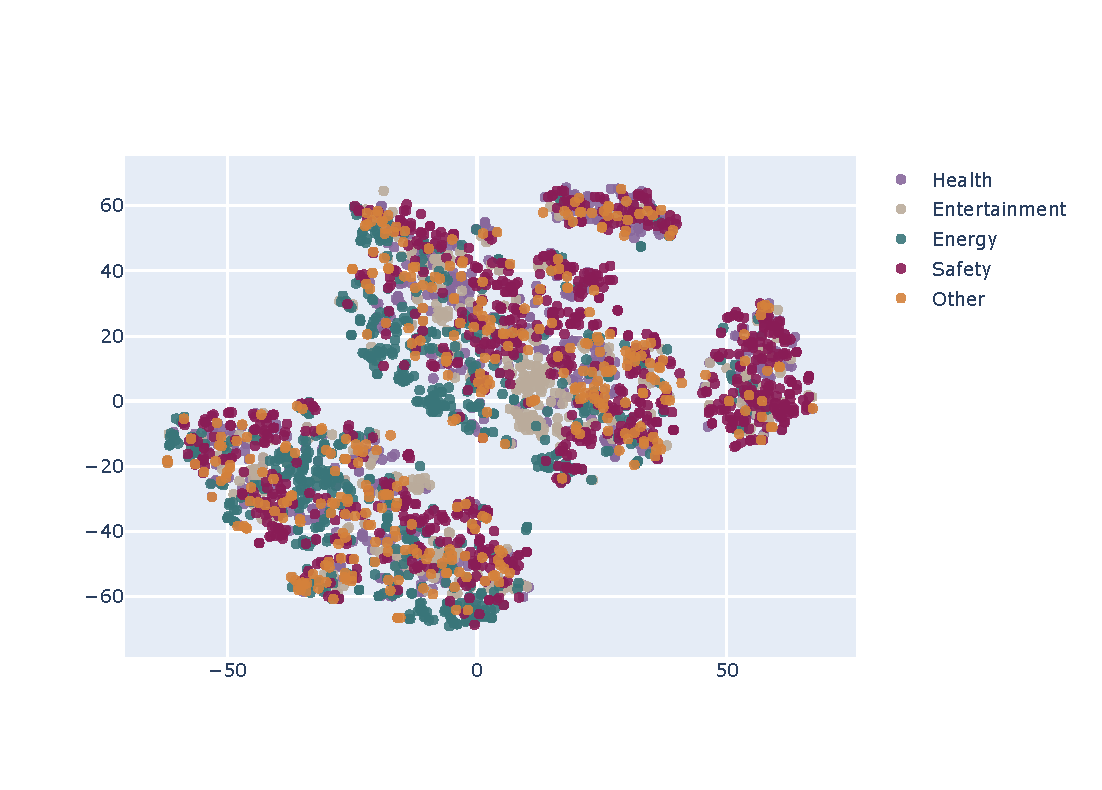
\includegraphics[width=0.49\textwidth]{figures/wmd_pretrained.pdf}}
    \caption{Results of the Word Mover's Distance}
    \label{fig:wmd-comparison}
\end{figure}
\FloatBarrier
% section analysis (end)